\documentclass[tikz]{standalone}
\usepackage{amsmath}
\usepackage{tikz}

\begin{document}

\begin{center}
\begin{figure}[h!]
\centering
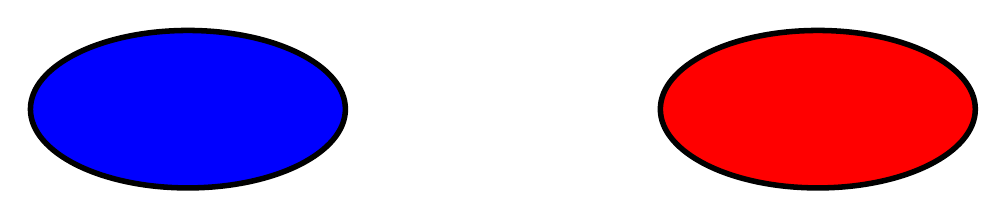
\begin{tikzpicture}
  % Blue ellipse on the left
  \draw[fill=blue, line width=2pt] (-4, 0) ellipse [x radius=2cm, y radius=1cm];

  % Red ellipse on the right
  \draw[fill=red, line width=2pt] (4, 0) ellipse [x radius=2cm, y radius=1cm];
\end{tikzpicture}
\caption{Visualization of two selected random sample from UTSG (left) and UTM (right)}
\end{figure}
\end{center}

\end{document}